\chapter{Related Work}
\label{chap:related_work}

This chapter reviews the main prior work on which this thesis builds. Section~\ref{sec:rw_causal_qa} introduces causal question answering and distinguishes between text-based and graph-based approaches. Section~\ref{sec:rw_causal_graphs} discusses causal knowledge graphs, their
construction, and their properties. Subsections~\ref{sec:rw_causenet} and~\ref{sec:rw_causalbank} present CauseNet and the Cause Effect Graph (CEG), the causal graph resources used in this work. Section 3.3 discusses the current state of the art in causal graph traversal, a reinforcement learning (RL) approach that addresses the same binary causal question answering task and therefore provides the most relevant point of comparison for this thesis. Finally, Section~\ref{sec:rw_learned_heuristics} reviews prior work on learned heuristics for $A^*$ search and discusses how it relates to the causal graph traversal setting considered in this thesis.

\section{Causal Question Answering}
\label{sec:rw_causal_qa}

Causal questions concern why events occur, what consequences they produce, whether one event causes another, and how outcomes would differ under interventions or counterfactual conditions~\cite{bondarenko:2022,wang:2024}. They therefore cover a range of tasks, from identifying causes and effects to reasoning about causal direction and hypothetical outcomes. The task is relevant in practice, as \citet{bondarenko:2022} estimate that at least $5\%$ of search-engine queries are causal. This thesis focuses on binary causal questions of the form ``Does $A$ cause $B$?''

Methods for causal question answering can broadly be divided into text-based and graph-based approaches. Text-based methods infer causal relationships from patterns, retrieved evidence, statistical associations, or neural language models. Although large language models perform well on some causal reasoning benchmarks~\cite{kiciman:2024}, controlled evaluations report only a preliminary understanding of causal graphs~\cite{chen:2024}, frequent confusion between causal and temporal relations~\cite{miliani:2025}, and substantial drops in effectiveness on fresh, nearly unseen data~\cite{chi:2024}. These findings suggest that current models often recall learned causal associations more reliably than they perform systematic causal reasoning~\cite{wu:2024}. Graph-based approaches instead operate on explicitly represented causal relationships, enabling algorithmic reasoning through methods such as graph traversal.

\section{Causal Knowledge Graphs}
\label{sec:rw_causal_graphs}

Knowledge graphs provide structured representations of entities or concepts and their relationships. General knowledge graphs such as \mbox{Wikidata}~\cite{vrandecic:2014}, \mbox{DBpedia}~\cite{auer:2007}, and ConceptNet~\cite{speer:2017} cover diverse relation types, whereas causal knowledge graphs focus specifically on cause--effect relationships.

Causal knowledge graphs may be created manually or automatically. Manual construction provides greater control over relationship quality but scales poorly, whereas automatic extraction enables large-scale coverage at the cost of increased noise. Prominent automatically extracted general-domain examples are CauseNet~\cite{heindorf:2020} and CEG~\cite{li:2020}. In contrast, domain-specific resources provide more constrained vocabularies and richer domain context at the cost of narrower coverage~\cite{kilicoglu:2012,garg:2025}. Causal knowledge graphs also differ in their level of normalization. Strongly normalized resources represent entities in structured and canonical forms, whereas weakly normalized resources represent textual concepts, phrases, or lexical terms more directly. CauseNet uses textual expressions as graph nodes, whereas CEG represents causal relationships between lemmatized terms rather than canonical entities~\cite{heindorf:2020,li:2020}. Strong normalization improves consistency and reduces duplication, while weak normalization preserves a broader range of linguistic expressions at the cost of greater ambiguity.

These characteristics influence both the quality and scale of causal knowledge graphs. In large, automatically constructed graphs, their size, noise, and weakly normalized representations can make efficient and reliable graph traversal particularly challenging.

\subsection{CauseNet}
\label{sec:rw_causenet}

CauseNet~\cite{heindorf:2020} is a large-scale causal knowledge graph containing millions of cause--effect relationships extracted from web data. It was constructed by identifying linguistic patterns that express causality and applying them to semi-structured and unstructured text sources. The resulting graph contains over $11$ million causal relationships with an estimated precision of approximately $83\%$. Each directed edge connects two textual concepts and contains provenance information that allows the represented causal relationship to be traced back to its source sentence. Since the graph is constructed automatically, it contains noisy and potentially spurious relationships. CauseNet therefore also provides a high-precision subset containing approximately $200{,}000$ relationships with a reported precision of $96\%$~\cite{heindorf:2020}. The full graph offers broader coverage, whereas the high-precision subset prioritizes relationship quality. Figure~\ref{fig:causenet_example} shows an example excerpt from CauseNet.

\begin{figure}[htbp]
    \centering
    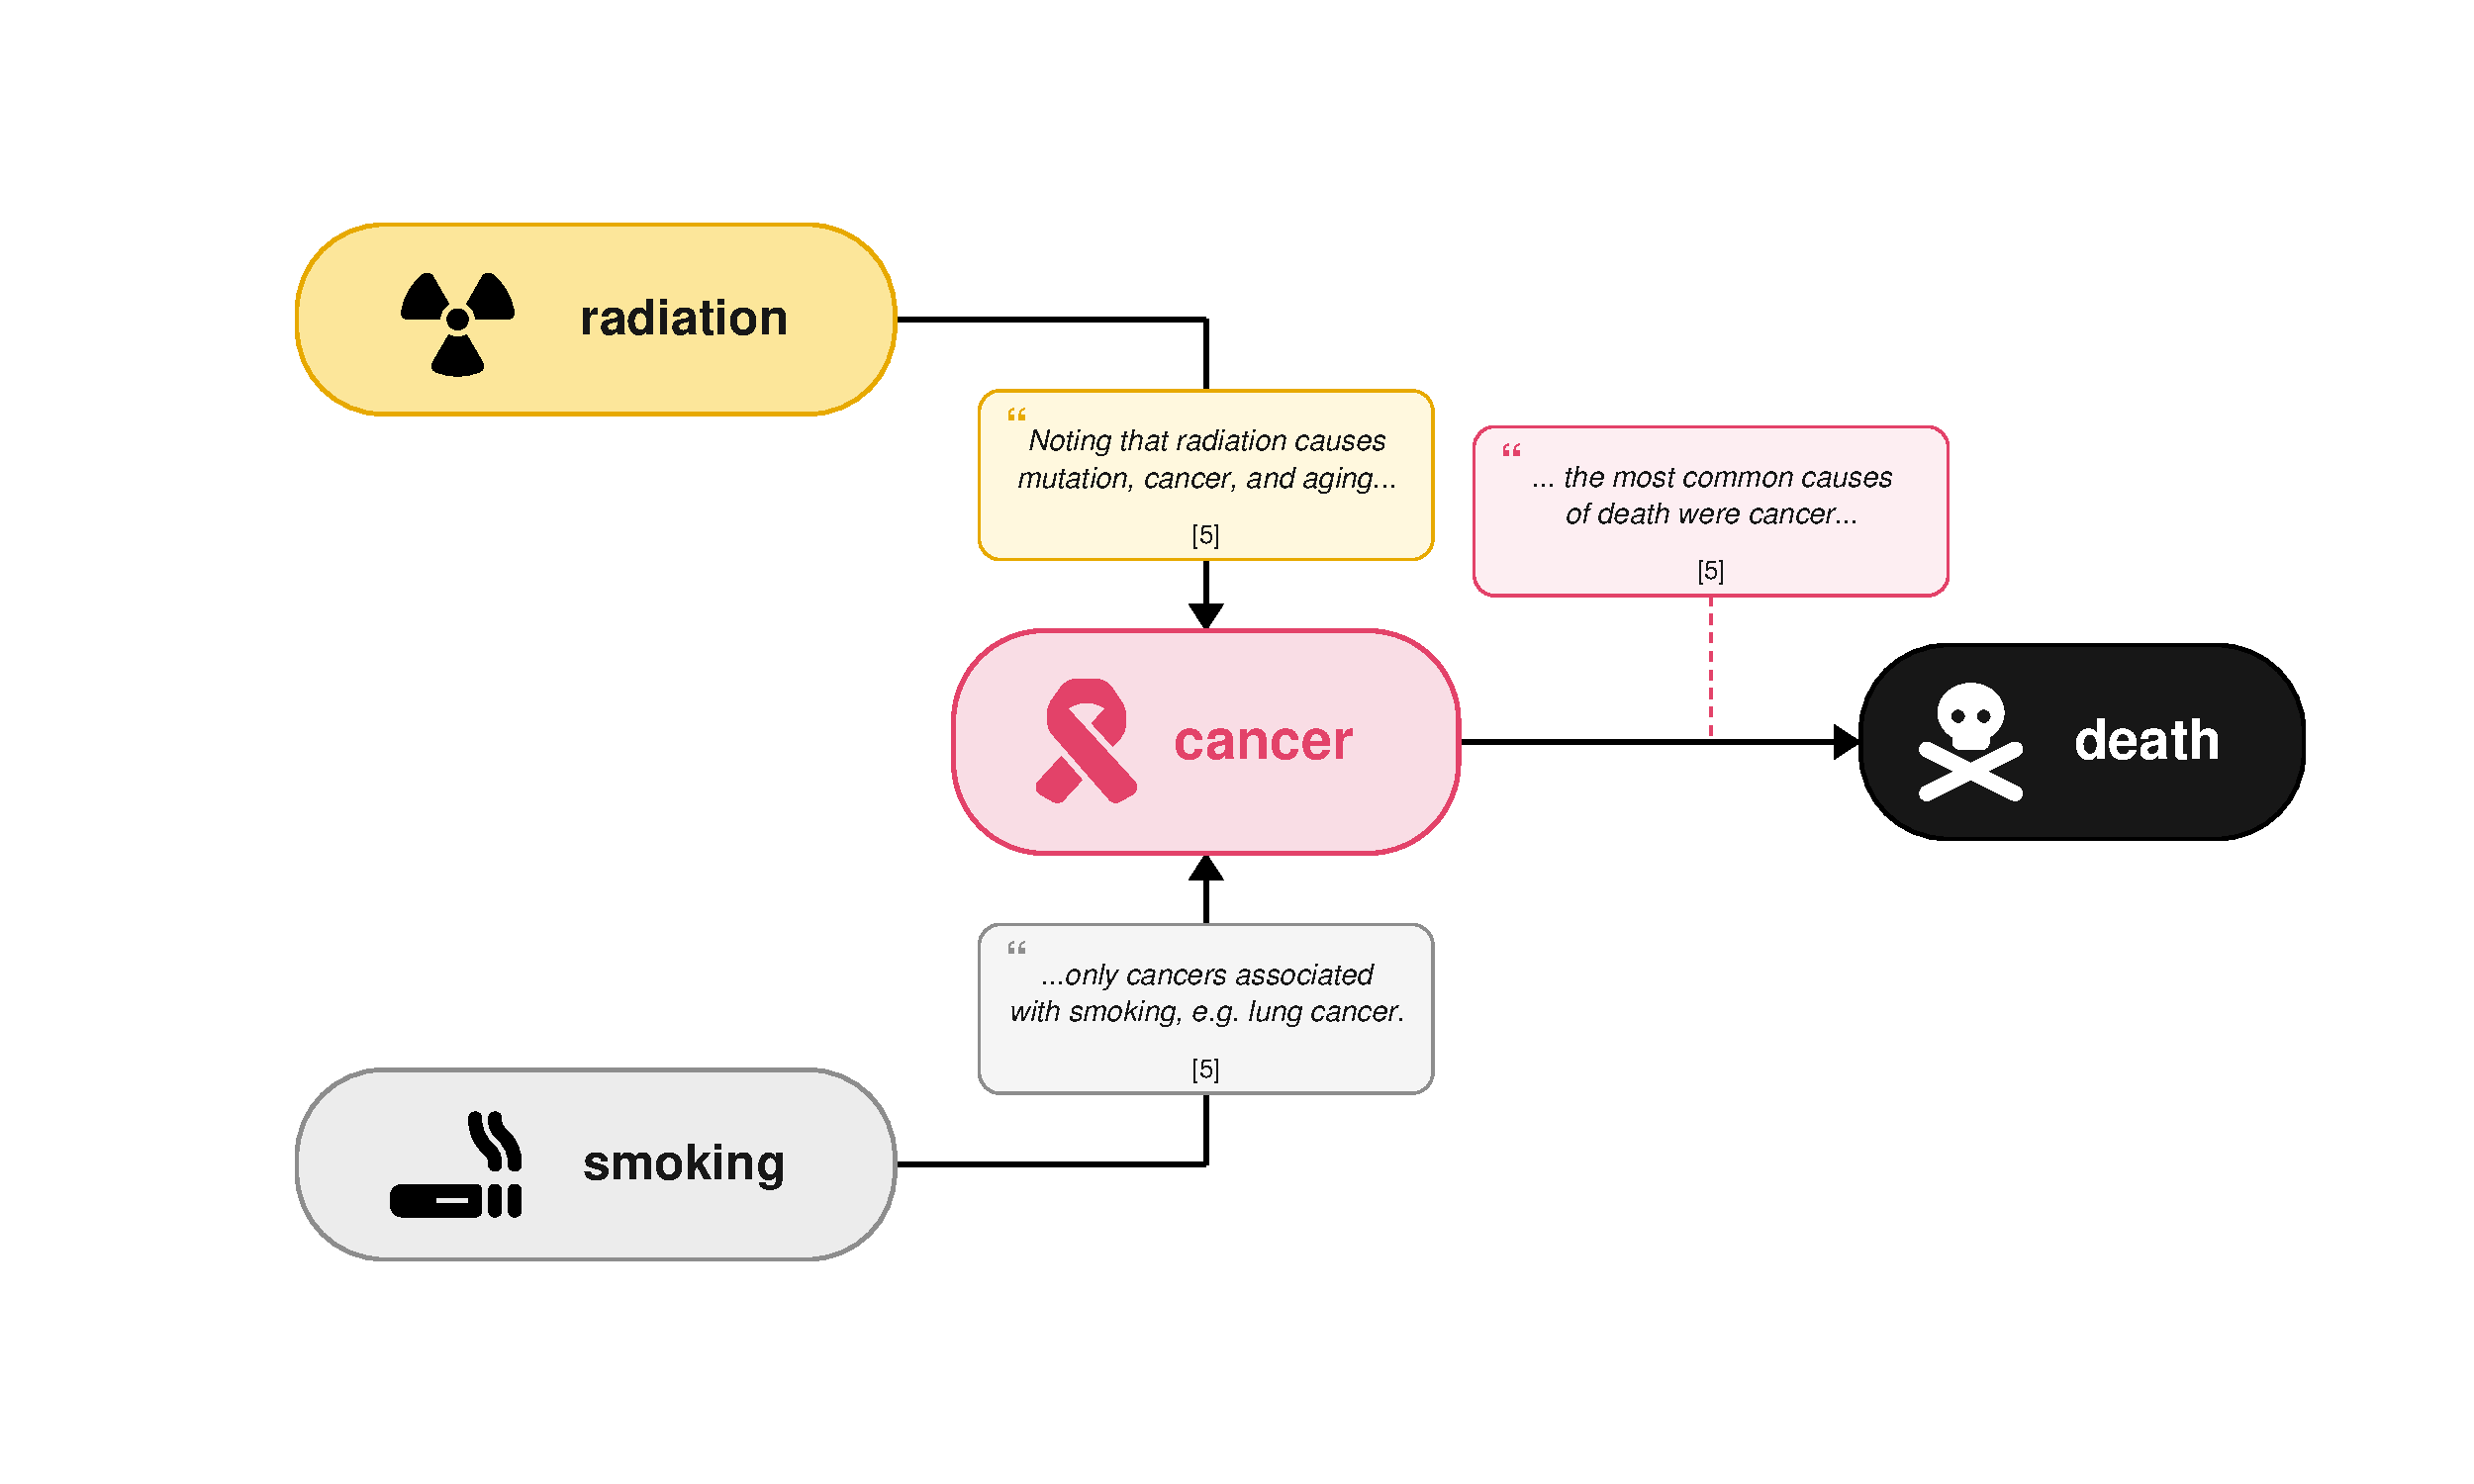
\includegraphics[width=1\linewidth]{figures/causenet.pdf}
    \caption{Example excerpt from CauseNet showing causal relations between concepts such as radiation, smoking, cancer, and death~\cite{heindorf:2020}.}
    \label{fig:causenet_example}
\end{figure}

\subsection{CausalBank and CEG}
\label{sec:rw_causalbank}

\citet{li:2020} introduce two related open-domain causal resources extracted automatically from the English Common Crawl corpus, namely CausalBank and CEG. CausalBank is a sentence-level corpus containing approximately $314$ million cause--effect pairs identified using lexical patterns that explicitly express causal relationships. CEG aggregates these extracted relationships into a directed graph between lemmatized terms. As this thesis investigates graph traversal, it uses CEG rather than the sentence-level CausalBank corpus. Each edge records the occurrence frequency of the corresponding term pair together with necessity and sufficiency causality scores. \citeauthor{li:2020} report approximately $89.1$ million relationships after filtering those occurring five times or less~\cite{li:2020}.

\section{RL Agent for Graph Traversal}
\label{sec:rw_rl}

\citet{bluebaum:2024} propose a reinforcement learning (RL) approach to binary causal question answering through graph traversal. Their agent is trained on CauseNet to learn a policy that maps the query and current graph node to a distribution over neighboring nodes. During inference, multiple paths are sampled, and a causal relationship is predicted if and only if one reaches the target node. By directing traversal toward promising neighbors, the approach reduces the number of explored nodes by up to $99\%$ compared with BFS while maintaining comparable accuracy~\cite{bluebaum:2024}. Despite these gains, the method requires training an RL agent and repeatedly evaluating its policy during traversal, resulting in additional computational overhead.

\section{Learned Heuristics for Search}
\label{sec:rw_learned_heuristics}

Informed search algorithms such as $A^*$ rely on heuristic functions to estimate
the remaining cost from a current state to the goal. Designing effective
heuristics manually often requires substantial domain knowledge and
problem-specific experimentation, which has motivated approaches that learn
these estimates from data. \citet{numeroso:2022} propose a
neural method for learning consistent heuristic functions that can be integrated directly into $A^*$ search. On synthetic pathfinding tasks, their learned heuristics reduce search effort compared with Dijkstra's algorithm while preserving optimality. This thesis instead investigates learned heuristics for binary causal question answering over large-scale causal knowledge graphs.
